\documentclass[12pt]{article}
\usepackage{graphicx}
\usepackage{enumitem}
\usepackage{amsmath}
\usepackage{gvv-book}
\usepackage{gvv}

\title{\textbf{4.10.3}}
\author{\textbf{Aditya Mishra- EE25BTECH}}
\date{September 30, 2025}

\begin{document}

\maketitle

\section*{Question}

Find the vector equation of the plane passing through the intersection of the planes
\[
\vec{r} \cdot (\hat{i} + \hat{j} + \hat{k}) = 6 \quad \text{and} \quad \vec{r} \cdot (2\hat{i} + 3\hat{j} + 4\hat{k}) = -5,
\]
and the point $(1, 1, 1)$.


\section*{Solution}

Given planes:
\[
\vec{n_1}^\top \vec{x} = c_1, \quad \vec{n_2}^\top \vec{x} = c_2,
\]
with point $\vec{P}$.


General solution for the plane passing through the intersection:
\[
\vec{n_1}^\top \vec{x} - c_1 + \lambda(\vec{n_2}^\top \vec{x} - c_2) = 0
\]
where
\[
\lambda = \frac{c_1 - \vec{n_1}^\top \vec{P}}{\vec{n_2}^\top \vec{P} - c_2}
\]

\bigskip
Given:
\[
\vec{n_1} = \myvec{1 \\ 1 \\ 1},\quad c_1 = 6, \quad
\vec{n_2} = \myvec{2 \\ 3 \\ 4},\quad c_2 = -5, \quad
\vec{P} = \myvec{1 \\ 1 \\ 1}.
\]

Evaluate:
\[
\vec{n_1}^\top \vec{P} = 3,\quad \vec{n_2}^\top \vec{P} = 9
\]
\[
\lambda = \frac{6-3}{9+5} = \frac{3}{14}
\]

Substituting all into the general family and simplifying:
\[
\vec{n_1}^\top \vec{x} - 6 + \frac{3}{14}(\vec{n_2}^\top \vec{x} + 5) = 0
\]


That is,
\[
\myvec{\frac{20}{14} \\ \frac{23}{14} \\ \frac{26}{14}}^\top \vec{x} = \frac{69}{14}
\]

Or, in simplest integer form, the equation of plane is:
\[
\boxed{
(20\quad 23\quad 26) \vec{x} = 69
}
\]
\section*{Plot}
\begin{figure}[H]
    \centering
    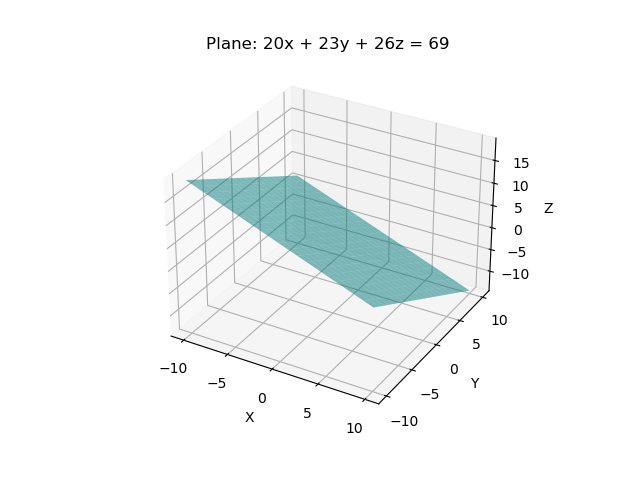
\includegraphics[width=1\columnwidth]{Figs/Figure.png}
\end{figure}

\end{document}

